\documentclass[11pt,a4paper]{article}
%%%%%%%%%%%%%%%%%%%%%%%%% Credit %%%%%%%%%%%%%%%%%%%%%%%%

% template ini dibuat oleh martin.manullang@if.itera.ac.id untuk dipergunakan oleh seluruh sivitas akademik itera.

%%%%%%%%%%%%%%%%%%%%%%%%% PACKAGE starts HERE %%%%%%%%%%%%%%%%%%%%%%%%
\usepackage{graphicx}
\usepackage{caption}
\usepackage{microtype}
\captionsetup[table]{name=Tabel}
\captionsetup[figure]{name=Gambar}
\usepackage{tabulary}
\usepackage{minted}
% \usepackage{amsmath}
\usepackage{fancyhdr}
% \usepackage{amssymb}
% \usepackage{amsthm}
\usepackage{placeins}
% \usepackage{amsfonts}
\usepackage{graphicx}
\usepackage[all]{xy}
\usepackage{tikz}
\usepackage{verbatim}
\usepackage[left=2cm,right=2cm,top=3cm,bottom=2.5cm]{geometry}
\usepackage{hyperref}
\hypersetup{
    colorlinks,
    linkcolor={red!50!black},
    citecolor={blue!50!black},
    urlcolor={blue!80!black}
}
\usepackage{caption}
\usepackage{subcaption}
\usepackage{multirow}
\usepackage{psfrag}
\usepackage[T1]{fontenc}
\usepackage[scaled]{beramono}
% Enable inserting code into the document
\usepackage{listings}
\usepackage{xcolor} 
% custom color & style for listing
\definecolor{codegreen}{rgb}{0,0.6,0}
\definecolor{codegray}{rgb}{0.5,0.5,0.5}
\definecolor{codepurple}{rgb}{0.58,0,0.82}
\definecolor{backcolour}{rgb}{0.95,0.95,0.92}
\definecolor{LightGray}{gray}{0.9}
\lstdefinestyle{mystyle}{
	backgroundcolor=\color{backcolour},   
	commentstyle=\color{green},
	keywordstyle=\color{codegreen},
	numberstyle=\tiny\color{codegray},
	stringstyle=\color{codepurple},
	basicstyle=\ttfamily\footnotesize,
	breakatwhitespace=false,         
	breaklines=true,                 
	captionpos=b,                    
	keepspaces=true,                 
	numbers=left,                    
	numbersep=5pt,                  
	showspaces=false,                
	showstringspaces=false,
	showtabs=false,                  
	tabsize=2
}
\lstset{style=mystyle}
\renewcommand{\lstlistingname}{Kode}
%%%%%%%%%%%%%%%%%%%%%%%%% PACKAGE ends HERE %%%%%%%%%%%%%%%%%%%%%%%%


%%%%%%%%%%%%%%%%%%%%%%%%% Data Diri %%%%%%%%%%%%%%%%%%%%%%%%
\newcommand{\student}{\textbf{Eric Arwido Damanik (122140157)}}
\newcommand{\course}{\textbf{Pengolahan Sinyal Digital (IF3024)}}
\newcommand{\assignment}{\textbf{xxx}}

%%%%%%%%%%%%%%%%%%% using theorem style %%%%%%%%%%%%%%%%%%%%
\newtheorem{thm}{Theorem}
\newtheorem{lem}[thm]{Lemma}
\newtheorem{defn}[thm]{Definition}
\newtheorem{exa}[thm]{Example}
\newtheorem{rem}[thm]{Remark}
\newtheorem{coro}[thm]{Corollary}
\newtheorem{quest}{Question}[section]
%%%%%%%%%%%%%%%%%%%%%%%%%%%%%%%%%%%%%%%%
\usepackage{lipsum}%% a garbage package you don't need except to create examples.
\usepackage{fancyhdr}
\pagestyle{fancy}
\lhead{Eric Arwido Damanik(122140157)}
\rhead{ \thepage}
\cfoot{\textbf{Program Pendeteksi Sinyal rPPG dan Sinyal Resipirasi}}
\renewcommand{\headrulewidth}{0.4pt}
\renewcommand{\footrulewidth}{0.4pt}

%%%%%%%%%%%%%%  Shortcut for usual set of numbers  %%%%%%%%%%%

\newcommand{\N}{\mathbb{N}}
\newcommand{\Z}{\mathbb{Z}}
\newcommand{\Q}{\mathbb{Q}}
\newcommand{\R}{\mathbb{R}}
\newcommand{\C}{\mathbb{C}}
\setlength\headheight{14pt}

%%%%%%%%%%%%%%%%%%%%%%%%%%%%%%%%%%%%%%%%%%%%%%%%%%%%%%%555
\begin{document}
\thispagestyle{empty}
\begin{center}
	\includegraphics[scale = 0.15]{Figure/ifitera-header.png}
	\vspace{0.1cm}
\end{center}
\noindent
\rule{17cm}{0.2cm}\\[0.3cm]
Nama Anggota: \student \hfill Tugas : Tugas Besar\\[0.1cm]
Mata Kuliah: \course \hfill Tanggal: 31 Mei 2025\\
\rule{17cm}{0.05cm}
\vspace{0.1cm}



%%%%%%%%%%%%%%%%%%%%%%%%%%%%%%%%%%%%%%%%%%%%% BODY DOCUMENT %%%%%%%%%%%%%%%%%%%%%%%%%%%%%%%%%%%%%%%%%%%%%
\section*{Program Pendeteksi Sinyal rPPG dan Sinyal Resipirasi}
\section{Pendahuluan}
    Proyek ini merupakan tugas akhir yang dikembangkan dalam rangka memenuhi sebagian persyaratan kelulusan mata kuliah Pengolahan Sinyal Digital (IF3024). Tugas ini berfokus pada perancangan dan implementasi sebuah sistem perangkat lunak yang mampu mengakuisisi dan menganalisis dua jenis sinyal fisiologis penting, yaitu sinyal respirasi (pernapasan) dan sinyal remote photoplethysmography (rPPG) secara real-time. Sumber input utama untuk sistem ini adalah video yang ditangkap langsung dari kamera web standar.\\
    Untuk memperoleh sinyal respirasi, program memanfaatkan kemampuan modul deteksi pose (Pose Estimation) dari pustaka MediaPipe. Secara spesifik, pergerakan vertikal dari landmark bahu pengguna dilacak dan dianalisis sebagai proksi untuk merepresentasikan siklus inspirasi dan ekspirasi selama proses pernapasan.\\
    Sementara itu, untuk ekstraksi sinyal rPPG yang kemudian digunakan untuk estimasi detak jantung, program menggunakan modul deteksi wajah (Face Detection) dari MediaPipe. Modul ini berfungsi untuk mengidentifikasi Region of Interest (ROI) pada wajah pengguna, dengan fokus utama pada area dahi. Perubahan subtil dalam intensitas warna kulit pada ROI tersebut, yang disebabkan oleh variasi volume darah akibat denyut jantung, dianalisis menggunakan algoritma Plane Orthogonal-to-Skin (POS) untuk mengkonversi sinyal RGB menjadi sinyal PPG mentah.

\section{Alat dan Bahan}
     Untuk menyelesaikan proyek ini, diperlukan beberapa alat dan bahan untuk membuat program yang dapat memperoleh sinyal rPPG dan sinyal respirasi secara non-kontak. Berikut merupakan alat dan bahan yang digunakan:
     
\subsection{Bahasa Pemograman}
      Dalam pengembangan program proyek ini, digunakan bahasa pemrograman \textbf{Python} karena memiliki dukungan library yang umum digunakan untuk proyek komputer visi.

\subsection{Library}
     Berikut merupakan library yang digunakan pada pengembangan proyek ini.
\begin{itemize}
    \item OpenCV: Untuk akuisisi dan pemrosesan gambar dari webcam.
    \item MediaPipe: Untuk deteksi pose (estimasi gerakan bahu untuk sinyal pernapasan) dan deteksi \item wajah (ROI untuk sinyal rPPG).
    \item NumPy: Untuk operasi numerik, terutama dalam pemrosesan sinyal.
    \item SciPy: Untuk fungsi pemrosesan sinyal seperti filter (Butterworth).
    \item PyQt6: Untuk membangun antarmuka pengguna grafis (GUI) aplikasi.
    \item PyQtGraph: Untuk menampilkan plot sinyal secara real-time di GUI.
    \item Pandas: Untuk manipulasi data, terutama saat membaca dan menulis file CSV.
    \item Matplotlib: Untuk menghasilkan plot ringkasan analisis sinyal yang disimpan sebagai gambar.
\end{itemize}

\subsection{Metode dan Algoritma}
     Berikut merupakan metode dan algortima yang digunakan pada pengembangan proyek ini.

\subsubsection{Sinyal Respirasi}
\begin{itemize}
    \item Akuisisi Sinyal Mentah : Pelacakan landmark bahu kiri dan kanan menggunakan MediaPipe Pose dan Perhitungan posisi vertikal rata-rata kedua bahu.
    \item Pemrosesan Sinyal Respirasi : Sinyal mentah difilter menggunakan filter low-pass Butterworth untuk menghilangkan noise dan komponen frekuensi tinggi yang tidak relevan, Kemudian dihitung menggunakan Fast Fourier Transform (FFT) pada segmen sinyal yang telah difilter.
\end{itemize}

\subsubsection{Sinyal Respirasi}
\begin{itemize}
    \item Akuisisi Sinyal Mentah : Menggunakan MediaPipe Face Detection untuk menentukan ROI pada dahi dan mengekstraksi nilai rata-rata channel RGB.
    \item Konversi ke Sinyal PPG : Sinyal RGB mentah diproses menggunakan Metode POS (Plane-Orthogonal-to-Skin) untuk menghasilkan sinyal PPG mentah.
    \item Pemrosesan Sinyal PPG : Sinyal PPG RGB mentah di proses menggunakan metode detrent untuk menghilangkan variasi frekuensi rendah kemudian difilter menggunakan filter bandpass Butterworth.
\end{itemize}
     

\section{Penjelasan}
    Program pada proyek ini dibagi menjadi dua modul, yaitu \texttt{main\_app.py} dan \texttt{signal\_proccesing.py}. Berikut adalah penjelasan mengenai alur kerja program yang dikembangkan dalam proyek ini:

\subsection{Instalasi Library}
     Agar dapat menjalankan program, pengguna dapat menambahkan beberapa library ke dalam python environment yang akan digunakan. Pengguna dapat mengunduh library yang digunakan menggunakan dua cara, yaitu:

\subsubsection{Menggunakan environment.yml}
     \begin{lstlisting}[language=Python, caption=Install Library/Pustaka menggunakan environment.yml,label={labelkode}]
     conda env create-f environment.yml
    \end{lstlisting}

\subsubsection{Menggunakan requirements.txt}
     \begin{lstlisting}[language=Python, caption=Install Library/Pustaka menggunakan requirements.txt,label={labelkode}]
     pip install-r requirements.txt
    \end{lstlisting}
    
\subsection{Modul \texttt{signal\_proccesing.py}}
     Modul ini berisi kumpulan fungsi yang spesifik untuk melakukan berbagai tahapan pemrosesan sinyal digital. Fungsi-fungsinya meliputi:
     
\subsubsection{Import Librabry}
     Berikut merupakan penjelasan dari Import Library pada modul \texttt{signal\_proccesing.py}.
     \begin{lstlisting}[language=Python, caption=Import Library pada modul \texttt{signal\_proccesing.py},label={labelkode}]
     import numpy as np
     from scipy.signal import butter, filtfilt, find_peaks, detrend
    \end{lstlisting}

\subsubsection{Fungsi \texttt{detrant\_signal}}.
     \begin{lstlisting}[language=Python, caption=Fungsi \texttt{detrant\_signal},label={labelkode}]
    def detrend_signal(signal_data, type='linear'):
    """
    Menghilangkan tren dari sinyal.
    'linear': Menghilangkan tren linear.
    'constant': Sama seperti mengurangi mean.
    """
    if signal_data.ndim > 1:
        detrended_signal = np.zeros_like(signal_data)
        for i in range(signal_data.shape[0]):
            detrended_signal[i, :] = detrend(signal_data[i, :], type=type)
        return detrended_signal
    else:
        return detrend(signal_data, type=type)
    \end{lstlisting}

\subsubsection{Fungsi \texttt{cpu\_POS}}.
     \begin{lstlisting}[language=Python, caption=Fungsi \texttt{cpu\_POS},label={labelkode}]
    def cpu_POS(rgb_signal, fps):
    """
    POS method on CPU using Numpy. This converts raw RGB signal to a pulse signal.
    Wang, W., den Brinker, A. C., Stuijk, S., & de Haan, G. (2016).
    """
    if rgb_signal.shape[1] < 2:
        return np.zeros(rgb_signal.shape[1])
        
    w = int(1.6 * fps)
    if rgb_signal.shape[1] < w:
        w = rgb_signal.shape[1]

    X = rgb_signal.T
    mean_color = np.mean(X, axis=0)
    diag_mean_color = np.diag(1 / (mean_color + 1e-9))
    Xn = np.matmul(X, diag_mean_color)
    Xn = Xn.T

    P = np.array([[0, 1, -1], [-2, 1, 1]])
    S = np.dot(P, Xn)
    
    H = np.zeros(S.shape[1])
    for i in range(S.shape[1] - w):
        S_window = S[:, i:i+w]
        S_std = np.std(S_window, axis=1)
        
        if S_std[1] < 1e-9:
            alpha = 0
        else:
            alpha = S_std[0] / S_std[1]
            
        H_window = S_window[0, :] + alpha * S_window[1, :]
        H[i:i+w] = H[i:i+w] + (H_window - np.mean(H_window))
        
    return H
    \end{lstlisting}
    
\subsubsection{Fungsi \texttt{filter\_sinyal\_respirasi}}.
     \begin{lstlisting}[language=Python, caption=Fungsi \texttt{filter\_sinyal\_respirasi},label={labelkode}]
    def filter_sinyal_respirasi(data, sample_rate, cutoff_freq=0.8, order=2):
    """Filter sinyal respirasi menggunakan low-pass filter."""
    if len(data) < 20:
        return np.array(data)

    nyquist = 0.5 * sample_rate
    if not (0 < cutoff_freq < nyquist):
        return np.array(data)
        
    b, a = butter(order, cutoff_freq, btype='low', fs=sample_rate)
    return filtfilt(b, a, data)
    \end{lstlisting}

\subsubsection{Fungsi \texttt{hitung\_laju\_napas}}.
     \begin{lstlisting}[language=Python, caption=Fungsi \texttt{hitung\_laju\_napas},label={labelkode}]
    def hitung_laju_napas(sinyal, sample_rate):
    """Menghitung laju napas dari sinyal menggunakan FFT."""
    if len(sinyal) < int(2 * sample_rate) or sample_rate <= 0:
        return "N/A"
    
    sinyal_tanpa_dc = sinyal - np.mean(sinyal)
    fft_result = np.fft.fft(sinyal_tanpa_dc)
    freqs = np.fft.fftfreq(len(sinyal), 1.0 / sample_rate)
    
    idx = np.where((freqs >= 0.1) & (freqs <= 0.8)) 
    if len(idx[0]) == 0:
        return "N/A (Tidak ada frekuensi dominan di rentang napas)"
    
    dominant_freq_idx = idx[0][np.argmax(np.abs(fft_result[idx]))]
    dominant_freq = freqs[dominant_freq_idx]
    
    return f"{dominant_freq * 60:.1f} BPM"
    \end{lstlisting}

\subsubsection{Fungsi \texttt{bandpass\_filter\_rppg}}.
     \begin{lstlisting}[language=Python, caption=Fungsi \texttt{bandpass\_filter\_rppg},label={labelkode}]
     def bandpass_filter_rppg(data, sample_rate, lowcut=0.7, highcut=2.5, order=4):
    """Bandpass filter sinyal rPPG."""
    if len(data) < int(2 * sample_rate * (order + 1)) or sample_rate <=0: 
        return np.array(data)
    
    nyquist = 0.5 * sample_rate
    if not (0 < lowcut < nyquist and 0 < highcut < nyquist and lowcut < highcut):
        return np.array(data)

    b, a = butter(order, [lowcut, highcut], btype='band', fs=sample_rate)
    return filtfilt(b, a, data)
    \end{lstlisting}

\subsubsection{Fungsi \texttt{hitung\_detak\_jantung}}.
     \begin{lstlisting}[language=Python, caption=Fungsi \texttt{hitung\_detak\_jantung},label={labelkode}]
    def hitung_detak_jantung(raw_rgb_signal, fps):
    """
    Menghitung detak jantung dari sinyal RGB mentah.
    Langkah: RGB -> Detrend -> POS -> Bandpass Filter -> Cari Puncak.
    """
    if raw_rgb_signal.shape[1] < int(2 * fps) or fps <= 0:
        return "N/A (Kurang data atau FPS tidak valid)"

    detrended_rgb_signal = detrend_signal(raw_rgb_signal, type='linear')
    pulse_signal = cpu_POS(detrended_rgb_signal, fps)
    
    if len(pulse_signal) < int(2 * fps):
        return "N/A (Sinyal POS tidak cukup)"

    filtered_pulse = bandpass_filter_rppg(pulse_signal, fps)
    
    if len(filtered_pulse) < int(fps / 2.5) +1:
         return "N/A (Sinyal terfilter tidak cukup)"

    if np.std(filtered_pulse) > 1e-6:
        normalized_pulse = (filtered_pulse - np.mean(filtered_pulse)) / np.std(filtered_pulse)
        min_height_normalized = 0.5
        peaks, _ = find_peaks(normalized_pulse, height=min_height_normalized, distance=fps / 2.5)
    else:
        peaks = []

    durasi_detik_efektif = len(filtered_pulse) / fps
    if durasi_detik_efektif == 0: 
        return "N/A (Durasi efektif nol)"
    
    if len(peaks) > 1:
        bpm = (len(peaks) -1) / ((peaks[-1] - peaks[0]) / fps) * 60
    elif len(peaks) == 1 and durasi_detik_efektif > 0:
        bpm = 1 * (60 / durasi_detik_efektif)
    else:
        bpm = 0.0
        
    return f"{bpm:.1f} BPM"
    \end{lstlisting}
    
\subsection{Modul \texttt{main\_app.py}}
     Modul ini berfungsi sebagai program utama yang menjalankan aplikasi dengan antarmuka pengguna grafis (GUI). Tugasnya meliputi:

\subsubsection{Import Librabry}
     Berikut merupakan penjelasan dari Import Library pada modul \texttt{main\_app.py}.
     \begin{lstlisting}[language=Python, caption=Import Library pada modul \texttt{main\_app.py},label={labelkode}]
    import time
    import cv2
    import mediapipe as mp
    import numpy as np
    import os
    from datetime import datetime, timedelta
    import csv
    import pandas as pd
    import matplotlib.pyplot as plt
    
    import signal_proccesing as vp
    
    from PyQt6.QtWidgets import QApplication, QMainWindow, QWidget, QVBoxLayout, QHBoxLayout, QLabel, QPushButton
    from PyQt6.QtCore import QThread, pyqtSignal, Qt, QObject, QTimer
    from PyQt6.QtGui import QImage, QPixmap
    import pyqtgraph as pg
    from pyqtgraph.exporters import ImageExporter
    \end{lstlisting}

\subsubsection{Kelas WorkerSignals}.
     Kelas ini mendefinisikan sinyal-sinyal PyQt (pyqtSignal) yang digunakan untuk komunikasi antar-thread. Fungsinya meliputi:
     \begin{lstlisting}[language=Python, caption=Kelas WorkerSignals,label={labelkode}]
    class WorkerSignals(QObject):
        frame_update = pyqtSignal(np.ndarray)
        data_update = pyqtSignal(float, float, float)
        results_update = pyqtSignal(str, str)
        finished = pyqtSignal(list, list, list, list)
    \end{lstlisting}
    
\subsubsection{Kelas RealTimeSignalWorker}.
     Kelas ini berfungsi sebagai Worker thread untuk memproses sinyal real-time dari kamera. Fungsinya meliputi:
    \begin{lstlisting}[language=Python, caption=Kelas RealTimeSignalWorker,label={labelkode}]
    class RealTimeSignalWorker(QThread):
    """Worker thread untuk memproses sinyal real-time dari kamera"""
    def __init__(self, parent=None):
        super().__init__(parent)
        self.signals = WorkerSignals()
        self.is_running = True
        self.all_timestamps = []
        self.all_respiration_data = [] 
        self.all_rppg_rgb_data = []    
        self.all_live_g_minus_b_plot_data = []

    def run(self):
        """Main loop untuk capture dan proses video stream"""
        cap = cv2.VideoCapture(0)
        fps_aktual = cap.get(cv2.CAP_PROP_FPS)
        if not (fps_aktual and fps_aktual >= 1.0):
            print("Peringatan: FPS kamera tidak valid, diatur ke 30.0 FPS")
            fps_aktual = 30.0 
        else:
            print(f"Kamera FPS terdeteksi/diatur: {fps_aktual:.2f}")

        mp_pose = mp.solutions.pose.Pose(min_detection_confidence=0.5, min_tracking_confidence=0.5)
        mp_face = mp.solutions.face_detection.FaceDetection(model_selection=0, min_detection_confidence=0.5)

        start_time = time.time()
        last_results_update_time = start_time
        
        self.all_timestamps.clear()
        self.all_respiration_data.clear()
        self.all_rppg_rgb_data.clear()
        self.all_live_g_minus_b_plot_data.clear()

        while self.is_running:
            ret, frame = cap.read()
            if not ret:
                print("Gagal membaca frame dari kamera.")
                break

            frame = cv2.flip(frame, 1) 
            frame_height, frame_width, _ = frame.shape
            image_rgb_for_mediapipe = cv2.cvtColor(frame, cv2.COLOR_BGR2RGB)

            current_y_avg_respiration = 0.0
            current_mean_rgb_from_roi = np.array([0.0, 0.0, 0.0]) 
            live_g_minus_b_signal_value = 0.0 

            results_pose = mp_pose.process(image_rgb_for_mediapipe)
            if results_pose.pose_landmarks:
                landmarks = results_pose.pose_landmarks.landmark
                left_shoulder_idx = mp.solutions.pose.PoseLandmark.LEFT_SHOULDER.value
                right_shoulder_idx = mp.solutions.pose.PoseLandmark.RIGHT_SHOULDER.value
                if (len(landmarks) > max(left_shoulder_idx, right_shoulder_idx) and
                    landmarks[left_shoulder_idx].visibility > 0.5 and
                    landmarks[right_shoulder_idx].visibility > 0.5):
                    y_left = landmarks[left_shoulder_idx].y * frame_height
                    y_right = landmarks[right_shoulder_idx].y * frame_height
                    current_y_avg_respiration = (y_left + y_right) / 2.0
                    cv2.circle(frame, (int(landmarks[left_shoulder_idx].x * frame_width), int(y_left)), 5, (0, 255, 0), -1)
                    cv2.circle(frame, (int(landmarks[right_shoulder_idx].x * frame_width), int(y_right)), 5, (0, 255, 0), -1)

            results_face = mp_face.process(image_rgb_for_mediapipe)
            if results_face.detections:
                detection = results_face.detections[0] 
                bboxC = detection.location_data.relative_bounding_box 
                face_x_abs = int(bboxC.xmin * frame_width)
                face_y_abs = int(bboxC.ymin * frame_height)
                face_w_abs = int(bboxC.width * frame_width)
                face_h_abs = int(bboxC.height * frame_height)
                if face_w_abs > 0 and face_h_abs > 0:
                    forehead_roi_h = int(face_h_abs * 0.25) 
                    forehead_roi_w = int(face_w_abs * 0.50) 
                    forehead_roi_y = max(0, face_y_abs - ROI_DAHI_OFFSET_Y_KE_ATAS) 
                    forehead_roi_x = face_x_abs + int((face_w_abs - forehead_roi_w) / 2) 
                    forehead_roi_x_end = forehead_roi_x + forehead_roi_w
                    forehead_roi_y_end = forehead_roi_y + forehead_roi_h 
                    if (forehead_roi_y_end <= frame_height and forehead_roi_x_end <= frame_width and
                        forehead_roi_w > 0 and forehead_roi_h > 0):
                        forehead_roi_bgr_pixels = frame[forehead_roi_y:forehead_roi_y_end, forehead_roi_x:forehead_roi_x_end]
                        if forehead_roi_bgr_pixels.size > 0:
                            mean_bgr_in_roi = np.mean(forehead_roi_bgr_pixels, axis=(0,1))
                            current_mean_rgb_from_roi = np.array([mean_bgr_in_roi[2], mean_bgr_in_roi[1], mean_bgr_in_roi[0]])
                            cv2.rectangle(frame, (forehead_roi_x, forehead_roi_y), (forehead_roi_x_end, forehead_roi_y_end), (0,0,255), 2)
            
            current_elapsed_time = time.time() - start_time
            self.all_timestamps.append(current_elapsed_time)
            self.all_respiration_data.append(current_y_avg_respiration)
            self.all_rppg_rgb_data.append(current_mean_rgb_from_roi) 

            if np.any(current_mean_rgb_from_roi): 
                mean_intensity_roi = np.mean(current_mean_rgb_from_roi)
                if mean_intensity_roi > 1e-9: 
                    normalized_rgb_live = current_mean_rgb_from_roi / mean_intensity_roi
                    live_g_minus_b_signal_value = normalized_rgb_live[1] - normalized_rgb_live[2] 
            self.all_live_g_minus_b_plot_data.append(live_g_minus_b_signal_value)

            if (time.time() - last_results_update_time) >= UPDATE_HASIL_SETIAP:
                if len(self.all_timestamps) > 1:
                    num_ts_for_sr = min(len(self.all_timestamps), int(fps_aktual * 5)) 
                    effective_sample_rate = fps_aktual 
                    if num_ts_for_sr > 1:
                        calculated_sr = 1.0 / np.mean(np.diff(self.all_timestamps[-num_ts_for_sr:]))
                        if calculated_sr > 0: effective_sample_rate = calculated_sr
                    min_points_for_calc_rppg = int(effective_sample_rate * DURASI_KALKULASI_RR_BPM)
                    min_points_for_calc_resp = int(effective_sample_rate * DURASI_KALKULASI_RESP)
                    rr_str = "N/A"
                    if len(self.all_respiration_data) >= min_points_for_calc_resp:
                        data_resp_segment = self.all_respiration_data[-min_points_for_calc_resp:]
                        filtered_resp_segment = vp.filter_sinyal_respirasi(data_resp_segment, effective_sample_rate)
                        if len(filtered_resp_segment) >= min_points_for_calc_resp * 0.8 : 
                             rr_str = vp.hitung_laju_napas(filtered_resp_segment, effective_sample_rate)
                    bpm_str = "N/A"
                    if len(self.all_rppg_rgb_data) >= min_points_for_calc_rppg:
                        data_rppg_segment_list = self.all_rppg_rgb_data[-min_points_for_calc_rppg:]
                        valid_rgb_list = [rgb for rgb in data_rppg_segment_list if isinstance(rgb, np.ndarray) and rgb.shape == (3,)]
                        if len(valid_rgb_list) >= min_points_for_calc_rppg * 0.8: 
                            rgb_array_for_calc = np.array(valid_rgb_list).T 
                            if rgb_array_for_calc.ndim == 2 and rgb_array_for_calc.shape[0] == 3:
                                 bpm_str = vp.hitung_detak_jantung(rgb_array_for_calc, effective_sample_rate)
                    self.signals.results_update.emit(rr_str, bpm_str)
                    last_results_update_time = time.time()

            min_len_for_live_filter = int(fps_aktual * 0.5)
            if len(self.all_respiration_data) > min_len_for_live_filter:
                filtered_total_resp_for_plot = vp.filter_sinyal_respirasi(self.all_respiration_data, fps_aktual)
            else:
                filtered_total_resp_for_plot = self.all_respiration_data 
            if len(self.all_live_g_minus_b_plot_data) > min_len_for_live_filter:
                filtered_total_g_minus_b_for_plot = vp.bandpass_filter_rppg(self.all_live_g_minus_b_plot_data, fps_aktual, lowcut=0.7, highcut=2.5)
            else:
                filtered_total_g_minus_b_for_plot = self.all_live_g_minus_b_plot_data 
            self.signals.frame_update.emit(frame) 
            self.signals.data_update.emit(
                current_elapsed_time, 
                filtered_total_resp_for_plot[-1] if len(filtered_total_resp_for_plot) > 0 else 0.0, 
                filtered_total_g_minus_b_for_plot[-1] if len(filtered_total_g_minus_b_for_plot) > 0 else 0.0
            )
            
        self.signals.finished.emit(
            self.all_timestamps, self.all_respiration_data, self.all_rppg_rgb_data, self.all_live_g_minus_b_plot_data 
        )
        cap.release()
        if 'mp_pose' in locals() and mp_pose is not None: mp_pose.close()
        if 'mp_face' in locals() and mp_face is not None: mp_face.close()
        print("Worker thread selesai dan resource MediaPipe dilepaskan.")

    def stop(self):
        """Menghentikan worker thread dengan aman"""
        print("Perintah stop diterima oleh RealTimeSignalWorker.")
        self.is_running = False
    \end{lstlisting}
\subsubsection{Kelas MainWindow}.
     Kelas ini berfungsi sebagai Main window aplikasi GUI untuk monitoring sinyal rPPG dan Respirasi. Fungsinya meliputi:
    \begin{lstlisting}[language=Python, caption=Kelas RealTimeSignalWorker,label={labelkode}]
    class MainWindow(QMainWindow):
    """Main window aplikasi GUI untuk monitoring sinyal vital"""
    def __init__(self):
        super().__init__()
        self.is_running_capture = False 
        self.capture_start_time = 0 
        self.setWindowTitle("Real Time Heart Rate & Resp Signal GUI")
        self.setGeometry(100, 100, 1300, 700) 

        main_widget = QWidget()
        self.setCentralWidget(main_widget)
        main_layout = QHBoxLayout(main_widget)

        left_column_widget = QWidget()
        left_layout = QVBoxLayout(left_column_widget)
        
        self.video_feed_label = QLabel("Tekan 'Mulai' untuk menampilkan video feed")
        self.video_feed_label.setAlignment(Qt.AlignmentFlag.AlignCenter)
        self.video_feed_label.setStyleSheet("background-color: #2E2E2E; color: white; font-size: 16px; border: 1px solid #555;")
        self.video_feed_label.setMinimumSize(640, 480) 
        left_layout.addWidget(self.video_feed_label, 5) 

        bottom_controls_area = QWidget()
        bottom_controls_layout = QVBoxLayout(bottom_controls_area)
        
        self.duration_label = QLabel("Durasi: 00:00:00") 
        self.duration_label.setAlignment(Qt.AlignmentFlag.AlignCenter)
        self.duration_label.setStyleSheet("font-size: 14px; margin-bottom: 5px;")
        bottom_controls_layout.addWidget(self.duration_label)

        buttons_layout = QHBoxLayout() 
        self.start_button = QPushButton("Mulai Pengambilan Data")
        self.start_button.setStyleSheet("background-color: #4CAF50; color: white; padding: 8px; font-size:14px;")
        self.stop_button = QPushButton("Hentikan Pengambilan Data")
        self.stop_button.setStyleSheet("background-color: #F44336; color: white; padding: 8px; font-size:14px;")
        self.stop_button.setEnabled(False)
        buttons_layout.addWidget(self.start_button)
        buttons_layout.addWidget(self.stop_button)
        bottom_controls_layout.addLayout(buttons_layout)
        
        left_layout.addWidget(bottom_controls_area, 1)

        main_layout.addWidget(left_column_widget, 2) 

        right_column_widget = QWidget()
        right_layout = QVBoxLayout(right_column_widget)

        self.resp_plot_widget = pg.PlotWidget(title="<font size='4'>Sinyal Pernapasan (RR)</font>")
        self.resp_plot_widget.setLabel('bottom', 'Waktu (detik)')
        self.resp_plot_widget.setLabel('left', 'Amplitudo Gerakan Bahu (px)')
        self.resp_plot_widget.showGrid(x=True, y=True, alpha=0.3)
        self.resp_plot_widget.getPlotItem().getViewBox().invertY(True) 
        self.plot_curve_resp = self.resp_plot_widget.plot(pen=pg.mkPen('#00FFFF', width=2)) 
        right_layout.addWidget(self.resp_plot_widget)

        self.rppg_plot_widget = pg.PlotWidget(title="<font size='4'>Sinyal Detak Jantung (rPPG)</font>")
        self.rppg_plot_widget.setLabel('bottom', 'Waktu (detik)')
        self.rppg_plot_widget.setLabel('left', 'Amplitudo Sinyal G-B (dinormalisasi)') 
        self.rppg_plot_widget.showGrid(x=True, y=True, alpha=0.3)
        self.rppg_plot_widget.enableAutoRange(axis='y', enable=True) 
        self.plot_curve_rppg = self.rppg_plot_widget.plot(pen=pg.mkPen('#39FF14', width=2)) 
        right_layout.addWidget(self.rppg_plot_widget)
        
        results_info_layout = QHBoxLayout()
        self.rr_label = QLabel("Laju Napas: -")
        self.rr_label.setStyleSheet("font-size: 14px; font-weight: bold;")
        self.bpm_label = QLabel("Detak Jantung (via POS): -") 
        self.bpm_label.setStyleSheet("font-size: 14px; font-weight: bold;")
        results_info_layout.addWidget(self.rr_label)
        results_info_layout.addStretch()
        results_info_layout.addWidget(self.bpm_label)
        right_layout.addLayout(results_info_layout)

        main_layout.addWidget(right_column_widget, 1) 

        self.start_button.clicked.connect(self.start_signal_capture)
        self.stop_button.clicked.connect(self.stop_signal_capture)
        
        self.plot_timestamps_buffer, self.plot_resp_data_buffer, self.plot_rppg_data_buffer = [], [], []

        # Timer untuk update durasi
        self.duration_timer = QTimer(self)
        self.duration_timer.timeout.connect(self.update_duration_label)

    def update_duration_label(self):
        if self.is_running_capture and self.capture_start_time > 0:
            elapsed_seconds = int(time.time() - self.capture_start_time)
            # Format HH:MM:SS
            formatted_time = str(timedelta(seconds=elapsed_seconds))
            self.duration_label.setText(f"Durasi: {formatted_time}")
        else:
            self.duration_label.setText("Durasi: 00:00:00")


    def start_signal_capture(self):
        """Memulai capture dan processing sinyal dari kamera"""
        if self.is_running_capture:
            return
        self.is_running_capture = True
        self.capture_start_time = time.time() 
        self.duration_timer.start(1000) 
        self.update_duration_label() 

        self.start_button.setEnabled(False)
        self.stop_button.setEnabled(True)
        self.rr_label.setText("Laju Napas: Mengukur...")
        self.bpm_label.setText("Detak Jantung (via POS): Mengukur...")
        self.video_feed_label.setText("Memulai kamera...")
        
        self.plot_timestamps_buffer.clear()
        self.plot_resp_data_buffer.clear()
        self.plot_rppg_data_buffer.clear()
        self.plot_curve_resp.clear() 
        self.plot_curve_rppg.clear()

        self.signal_processing_worker = RealTimeSignalWorker()
        self.signal_processing_worker.signals.frame_update.connect(self.update_video_frame_display)
        self.signal_processing_worker.signals.data_update.connect(self.update_live_plots)
        self.signal_processing_worker.signals.results_update.connect(self.update_rr_bpm_results)
        self.signal_processing_worker.signals.finished.connect(self.on_capture_finished_save_results)
        self.signal_processing_worker.start()
        print("Thread RealTimeSignalWorker dimulai.")

    def stop_signal_capture(self):
        """Menghentikan capture dan processing sinyal"""
        self.duration_timer.stop() # Hentikan timer durasi
        if hasattr(self, 'signal_processing_worker') and self.is_running_capture:
            print("Perintah stop dikirim dari MainWindow ke RealTimeSignalWorker.")
            self.signal_processing_worker.stop()
            # Status is_running_capture akan di-set False di on_capture_finished_save_results
            
    def update_video_frame_display(self, cv_frame):
        """Update tampilan video feed di GUI"""
        rgb_image = cv2.cvtColor(cv_frame, cv2.COLOR_BGR2RGB)
        h, w, ch = rgb_image.shape
        bytes_per_line = ch * w
        qt_image = QImage(rgb_image.data, w, h, bytes_per_line, QImage.Format.Format_RGB888)
        self.video_feed_label.setPixmap(QPixmap.fromImage(qt_image).scaled(
            self.video_feed_label.size(), 
            Qt.AspectRatioMode.KeepAspectRatio, 
            Qt.TransformationMode.SmoothTransformation
        ))

    def update_live_plots(self, timestamp, resp_val, rppg_val):
        """Update plot real-time untuk sinyal pernapasan dan detak jantung"""
        self.plot_timestamps_buffer.append(timestamp)
        self.plot_resp_data_buffer.append(resp_val)
        self.plot_rppg_data_buffer.append(rppg_val)

        if len(self.plot_timestamps_buffer) > JUMLAH_DATA_PLOT:
            self.plot_timestamps_buffer.pop(0)
            self.plot_resp_data_buffer.pop(0)
            self.plot_rppg_data_buffer.pop(0)

        self.plot_curve_resp.setData(self.plot_timestamps_buffer, self.plot_resp_data_buffer)
        self.plot_curve_rppg.setData(self.plot_timestamps_buffer, self.plot_rppg_data_buffer)
        self.rppg_plot_widget.enableAutoRange(axis='y', enable=True)


    def update_rr_bpm_results(self, rr_str, bpm_str):
        """Update hasil pengukuran laju napas dan detak jantung di GUI"""
        self.rr_label.setText(f"Laju Napas: {rr_str}")
        self.bpm_label.setText(f"Detak Jantung (via POS): {bpm_str}")

    def on_capture_finished_save_results(self, all_timestamps, all_respiration_data, all_rppg_rgb_data, all_live_g_minus_b_plot_data):
        """Menyimpan hasil pengukuran ke file saat capture selesai"""
        print("Sinyal 'finished' diterima oleh MainWindow dari RealTimeSignalWorker.")
        self.is_running_capture = False # Penting untuk di-set di sini
        self.duration_timer.stop() # Pastikan timer durasi berhenti
        # self.duration_label.setText("Durasi: Selesai") # Atau biarkan nilai terakhir

        self.start_button.setEnabled(True)
        self.stop_button.setEnabled(False)
        self.video_feed_label.setText("Pengambilan data dihentikan. Tekan 'Mulai' lagi.")
        
        if len(all_timestamps) > 10: 
            if not os.path.exists(FOLDER_HASIL):
                try:
                    os.makedirs(FOLDER_HASIL)
                    print(f"Folder '{FOLDER_HASIL}' telah dibuat.")
                except OSError as e:
                    print(f"Gagal membuat folder '{FOLDER_HASIL}': {e}")
                    return 

            csv_file_path = self.save_raw_data_to_csv(all_timestamps, all_respiration_data, all_rppg_rgb_data) 
            
            if csv_file_path: 
                self.generate_and_save_matplotlib_summary_plots(csv_file_path)
        else:
            print("Tidak cukup data untuk disimpan atau di-plot.")
            
    def closeEvent(self, event):
        print("Menutup aplikasi...")
        self.duration_timer.stop() # Hentikan timer saat menutup aplikasi
        self.stop_signal_capture()
        if hasattr(self, 'signal_processing_worker'):
            self.signal_processing_worker.wait() 
        super().closeEvent(event)

    def save_raw_data_to_csv(self, timestamps, raw_respiration_y_data, raw_rppg_mean_rgb_data):
        """Menyimpan data mentah ke file CSV"""
        if not os.path.exists(FOLDER_HASIL):
            try:
                os.makedirs(FOLDER_HASIL)
            except OSError as e:
                print(f"Gagal membuat folder '{FOLDER_HASIL}' untuk CSV: {e}")
                return None
        timestamp_str = datetime.now().strftime("%Y%m%d_%H%M%S")
        csv_filename = os.path.join(FOLDER_HASIL, f"data_realtime_signal_{timestamp_str}.csv")
        try:
            with open(csv_filename, 'w', newline='') as csvfile:
                writer = csv.writer(csvfile)
                writer.writerow(['timestamp', 'raw_respiration_y_avg_shoulder', 
                                 'raw_roi_mean_r', 'raw_roi_mean_g', 'raw_roi_mean_b'])
                for i in range(len(timestamps)):
                    ts = timestamps[i]
                    resp_y = raw_respiration_y_data[i]
                    rgb_val = raw_rppg_mean_rgb_data[i]
                    if isinstance(rgb_val, np.ndarray) and rgb_val.shape == (3,):
                        r_val, g_val, b_val = rgb_val[0], rgb_val[1], rgb_val[2]
                    else: 
                        r_val, g_val, b_val = 0.0, 0.0, 0.0
                    writer.writerow([ts, resp_y, r_val, g_val, b_val])
            print(f"Data Sinyal Real-time disimpan ke CSV: {csv_filename}")
            return csv_filename
        except Exception as e:
            print(f"Gagal menyimpan data Sinyal Real-time ke CSV: {e}")
            return None

    def generate_and_save_matplotlib_summary_plots(self, csv_filepath):
        """Membuat dan menyimpan plot ringkasan menggunakan matplotlib"""
        print(f"Membuat plot Matplotlib ringkasan dari: {csv_filepath}")
        try:
            df = pd.read_csv(csv_filepath)
        except Exception as e:
            print(f"Gagal membaca CSV untuk plot Matplotlib: {e}")
            return
        if df.empty or len(df) <= 1:
            print("CSV kosong atau tidak cukup data, tidak bisa membuat plot Matplotlib ringkasan.")
            return
        timestamps_csv = df['timestamp'].values
        raw_respiration_y_csv = df['raw_respiration_y_avg_shoulder'].values 
        raw_r_csv = df['raw_roi_mean_r'].values
        raw_g_csv = df['raw_roi_mean_g'].values
        raw_b_csv = df['raw_roi_mean_b'].values
        if len(timestamps_csv) <= 1:
            print("Tidak cukup data timestamp di CSV untuk menghitung sample rate.")
            return
        csv_sample_rate = 1.0 / np.mean(np.diff(timestamps_csv))
        if csv_sample_rate <= 0: 
            print(f"Sample rate dari CSV tidak valid: {csv_sample_rate:.2f}. Menggunakan default 30Hz.")
            csv_sample_rate = 30.0 
        filtered_respiration_csv = vp.filter_sinyal_respirasi(raw_respiration_y_csv, csv_sample_rate)
        rr_result_csv = vp.hitung_laju_napas(filtered_respiration_csv, csv_sample_rate)
        print(f"Laju Napas (dari CSV): {rr_result_csv}")
        raw_rgb_signal_csv = np.array([raw_r_csv, raw_g_csv, raw_b_csv])
        bpm_result_csv = vp.hitung_detak_jantung(raw_rgb_signal_csv, csv_sample_rate)
        print(f"Detak Jantung (dari CSV via POS): {bpm_result_csv}")
        if raw_rgb_signal_csv.shape[1] > int(2 * csv_sample_rate): 
            detrended_rgb_csv = vp.detrend_signal(raw_rgb_signal_csv, type='linear')
            pulse_signal_pos_csv = vp.cpu_POS(detrended_rgb_csv, csv_sample_rate) 
            if pulse_signal_pos_csv is not None and len(pulse_signal_pos_csv) > 0:
                 filtered_rppg_csv_for_plot = vp.bandpass_filter_rppg(pulse_signal_pos_csv, csv_sample_rate)
            else:
                print("Sinyal POS dari CSV kosong atau tidak valid untuk plot Matplotlib.")
                filtered_rppg_csv_for_plot = np.zeros_like(timestamps_csv) 
        else:
            print("Tidak cukup data RGB di CSV untuk proses rPPG untuk plot Matplotlib.")
            filtered_rppg_csv_for_plot = np.zeros_like(timestamps_csv) 
        if len(filtered_respiration_csv) > 0:
            filtered_resp_plot_csv = filtered_respiration_csv - np.mean(filtered_respiration_csv)
        else:
            filtered_resp_plot_csv = np.zeros_like(timestamps_csv)
        fig_summary, axs_summary = plt.subplots(2, 1, figsize=(14, 9), sharex=True)
        base_filename_csv = os.path.splitext(os.path.basename(csv_filepath))[0]
        fig_summary.suptitle(f"Ringkasan Analisis Sinyal Real-time (Matplotlib) - {base_filename_csv}", fontsize=16)
        axs_summary[0].plot(timestamps_csv, filtered_resp_plot_csv, label=f'Sinyal Respirasi Terfilter (RR: {rr_result_csv})', color='c', linewidth=1.5)
        axs_summary[0].set_ylabel('Amplitudo Gerakan Bahu (px)')
        axs_summary[0].set_title('Analisis Sinyal Pernapasan (dari Data CSV)')
        axs_summary[0].legend(loc='upper right')
        axs_summary[0].grid(True, linestyle=':', alpha=0.6)
        stable_start_time_sec = 5.0 
        if len(timestamps_csv) > 0 and len(filtered_resp_plot_csv) > 0 and timestamps_csv[-1] > stable_start_time_sec:
            try:
                if np.any(timestamps_csv >= stable_start_time_sec):
                    stable_idx_start = np.argmax(timestamps_csv >= stable_start_time_sec)
                else: 
                    stable_idx_start = len(timestamps_csv) 
            except ValueError: 
                stable_idx_start = 0 
            if stable_idx_start < len(filtered_resp_plot_csv) - 1: 
                data_for_scaling = filtered_resp_plot_csv[stable_idx_start:]
                if len(data_for_scaling) > 1: 
                    min_val = np.min(data_for_scaling)
                    max_val = np.max(data_for_scaling)
                    padding = (max_val - min_val) * 0.1 
                    if padding < 0.5: padding = 0.5 
                    if (max_val - min_val) < 0.1: 
                        mean_stable_segment = np.mean(data_for_scaling)
                        axs_summary[0].set_ylim([mean_stable_segment - 2, mean_stable_segment + 2]) 
                        print(f"Info: Sinyal respirasi setelah {stable_start_time_sec}s hampir datar. Zoom ke +/- 2px.")
                    else:
                        axs_summary[0].set_ylim([min_val - padding, max_val + padding])
                        print(f"Info: Skala Y respirasi diatur ke [{min_val - padding:.2f}, {max_val + padding:.2f}] (berdasarkan data setelah {stable_start_time_sec}s).")
            else:
                print(f"Info: Tidak cukup data respirasi setelah {stable_start_time_sec}s untuk penyesuaian skala Y otomatis.")
        else:
            print("Info: Durasi data respirasi terlalu pendek atau data kosong untuk penyesuaian skala Y otomatis.")
        axs_summary[1].plot(timestamps_csv, filtered_rppg_csv_for_plot, label=f'Sinyal rPPG Terfilter (BPM via POS: {bpm_result_csv})', color='g', linewidth=1.5)
        axs_summary[1].set_ylabel('Amplitudo Sinyal POS Terfilter')
        axs_summary[1].set_title(f'Analisis Sinyal rPPG (Detak Jantung - dari Data CSV)')
        axs_summary[1].legend(loc='upper right')
        axs_summary[1].grid(True, linestyle=':', alpha=0.6)
        axs_summary[1].set_xlabel('Waktu (detik)')
        plt.tight_layout(rect=[0, 0.03, 1, 0.95]) 
        mpl_summary_plot_filename = os.path.join(FOLDER_HASIL, f"plot_matplotlib_ringkasan_signal_{base_filename_csv}.png")
        try:
            plt.savefig(mpl_summary_plot_filename)
            print(f"Plot Matplotlib ringkasan disimpan ke: {mpl_summary_plot_filename}")
        except Exception as e:
            print(f"Gagal menyimpan plot Matplotlib ringkasan: {e}")
        plt.close(fig_summary) 
    \end{lstlisting}

\section{Hasil}
     Berdasarkan hasil implementasi, program berhasil mendeteksi wajah dan bahu dengan menggunakan MediaPipe.
\begin{figure}[h]
    \centering
    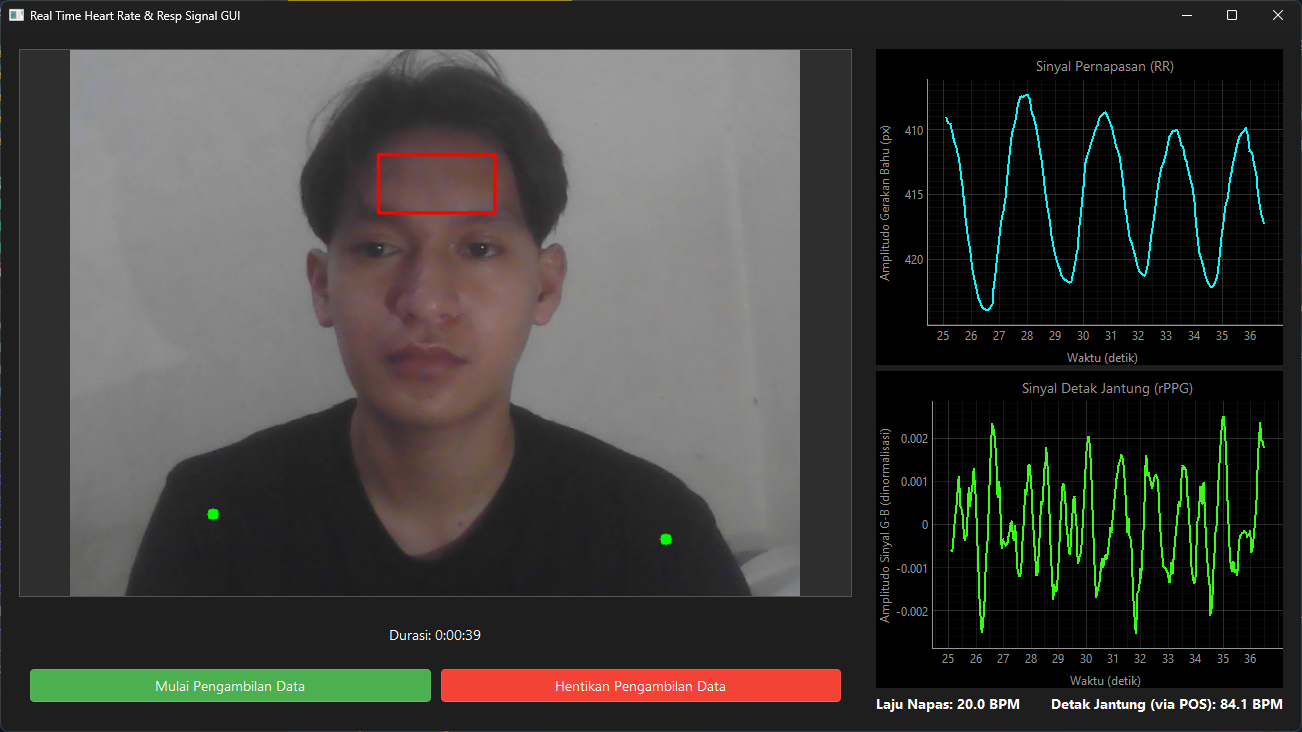
\includegraphics[width=0.8\textwidth]{Figure/Hasil_GUI.png}
    \caption{Hasil Deteksi Program}
    \label{fig:my_label}
\end{figure}\\

    Proyek ini berhasil mengembangkan sebuah program \textit{real-time} untuk mendeteksi sinyal respirasi dan rPPG menggunakan Python, OpenCV, dan MediaPipe. Sinyal respirasi diekstraksi melalui analisis pergerakan bahu menggunakan MediaPipe Pose, sementara sinyal rPPG diperoleh dari perubahan warna pada area dahi (\textit{Region of Interest}/ROI) dengan bantuan MediaPipe Face Detection, yang kemudian diproses menggunakan metode POS (\textit{Plane-Orthogonal-to-Skin}).\\
    Sinyal mentah yang diperoleh selanjutnya diproses dalam modul \texttt{signal\_processing.py}, yang mencakup tahapan \textit{detrending}, penyaringan menggunakan filter Butterworth (low-pass untuk sinyal respirasi dan band-pass untuk sinyal rPPG), serta estimasi laju pernapasan (\textit{Respiratory Rate}/RR) melalui analisis FFT, dan estimasi detak jantung (\textit{Beats Per Minute}/BPM) melalui deteksi puncak (\textit{peak detection}).\\
    Aplikasi ini dilengkapi dengan antarmuka pengguna grafis (GUI) yang dibangun menggunakan PyQt6 dan PyQtGraph. GUI ini menampilkan video secara langsung, visualisasi sinyal \textit{real-time}, serta hasil estimasi nilai RR dan BPM. Selain itu, program juga menyediakan fitur untuk menyimpan data sinyal mentah ke dalam file CSV dan menyimpan grafik hasil analisis dalam format gambar untuk keperluan dokumentasi atau analisis lanjutan.



\section{Referensi dan Daftar Pustaka}
Ini bagian yang sedikit \textit{tricky}. Anda harus memasukkan daftar pustaka anda ke sebuah file berekstensi .bib di bagian kiri dari overleaf ini. Konten dot bib ini dapat anda export dengan mudah, entah itu dari google scholar, mendeley, ataupun manajemen sitasi lainnya.\\\\
Cara penggunaanya pun cukup mudah. Misalnya saat ini saya ingin mensitasi salah satu dokumen yang ada, misalnya wikipedia, saya cukup menuliskan $\backslash${\tt{cite}} yang berisikan cite-key dari entri yang ada di file.bib \cite{Wikipedia_contributors2021-bb}. Contoh lain menuliskan sitasi adalah sebagai berikut \cite{Name2018-hd}.

\newpage
\bibliographystyle{IEEEtran}
\bibliography{Referensi}
\end{document}